\documentclass[crop,tikz]{standalone}

\usepackage[utf8]{inputenc}
% 'crop' is the default for v1.0, before it was 'preview'
%\usetikzlibrary{...}% tikz package already loaded by 'tikz' option

%The idea behind this file is that it will be used to store all the maths-related macros that I concoct; so that I can import all the commands by \input{this file} in the preamble of any file that I want to use them in.
%This should make the top-level files look a lot cleaner, and the preamble much shorter!

\usepackage{amssymb}
\usepackage{amsmath}

%theorems and lemma etc setup using amsthm
\usepackage{amsthm}
\newcommand{\tstk}[1]{\textbf{#1} \newline}
\theoremstyle{definition}
\newtheorem{definition}{Definition}[section]
\theoremstyle{plain}
\newtheorem{theorem}{Theorem}[section]
\theoremstyle{plain}
\newtheorem{lemma}[theorem]{Lemma}
\theoremstyle{plain}
\newtheorem{prop}[theorem]{Proposition}

\allowdisplaybreaks %allows equations in the same align environment to split over multiple pages.

%begin the macros via newcommand. Try to group them up reasonably!

%standard sets
\newcommand{\naturals}{\mathbb{N}}			%natural numbers
\newcommand{\integers}{\mathbb{Z}}			%integers
\newcommand{\rationals}{\mathbb{Q}}			%rational numbers
\newcommand{\reals}{\mathbb{R}}				%real numbers
\newcommand{\complex}{\mathbb{C}}			%complex numbers

%brackets and norms
\newcommand{\bracs}[1]{\left( #1 \right)}				%encloses input in brackets
\newcommand{\sqbracs}[1]{\left[ #1 \right]}				%encloses input in square brackets
\newcommand{\clbracs}[1]{\left\{ #1 \right\}}			%encloses input in curly bracers
\newcommand{\abs}[1]{\lvert #1 \rvert}					%absolute value
\newcommand{\norm}[2]{\lvert\lvert #1 \rvert\rvert}		%norm (double line)

%function sets
\newcommand{\smooth}[1]{C^{\infty}\bracs{#1}}							%smooth functions
\newcommand{\ltwo}[2]{L^{2}\bracs{#1,\mathrm{d}#2}}						%general L^2 space
\newcommand{\gradSob}[2]{H^1_\mathrm{grad}\bracs{#1, \mathrm{d}#2}}		%gradient Sobolev space
\newcommand{\curlSob}[2]{H^1_\mathrm{curl}\bracs{#1, \mathrm{d}#2}}		%curl Sobolev space
\newcommand{\kSob}[2]{H^1_{k,\mathrm{curl}}\bracs{#1, \mathrm{d}#2}}	%k-curl Sobolev space

%grad and curl sets
\newcommand{\gradZero}[2]{\mathcal{G}_{ #1, \mathrm{d}#2}\bracs{0}}		%gradients of zero for domain #1 with measure #2
\newcommand{\curlZero}[2]{\mathcal{C}_{ #1, \mathrm{d}#2}\bracs{0}}	%curls of zero for domain #1 with measure #2

%derivatives and grad-like symbols
\newcommand{\diff}[2]{\dfrac{\mathrm{d}#1}{\mathrm{d}#2}}			%complete derivative d#1/d#2
\newcommand{\pdiff}[2]{\dfrac{\partial #1}{\partial #2}}			%partial derivative p#1/p#2
\newcommand{\ddiff}[2]{\dfrac{\mathrm{d}^2 #1}{\mathrm{d}^2 #2}}	%2nd deriv
\newcommand{\grad}{\nabla}											%grad operator
\newcommand{\curl}[1]{\grad_{#1}\wedge}								%curl with measure subscript #1

%displaying integrals
\newcommand{\integral}[3]{\int_{#1}#2 \ \mathrm{d}#3}			%integral, domain #1, integrand #2, measure #3

%notation for variable use throughout the file
\newcommand{\dddom}{\widetilde{\Omega}}			%3D domain notation
\newcommand{\ddom}{\Omega}						%2D domain notation
\newcommand{\dddmes}{\widetilde{\mu}}			%3D measure
\newcommand{\ddmes}{\mu}						%2D measure

\newcommand{\graph}{\mathbb{G}}					%graph variable
	
\begin{document}

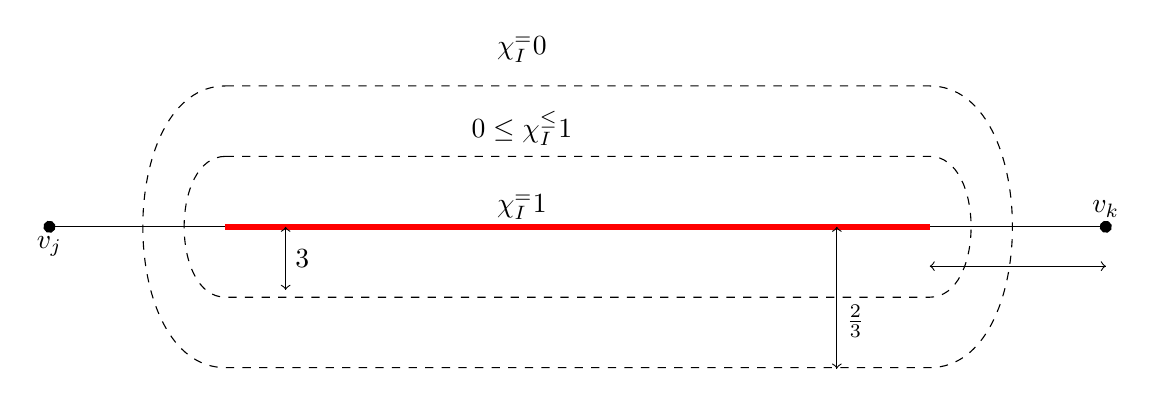
\begin{tikzpicture}
	\begin{scope}[scale=2, rotate=-26.565]
		\draw (0,0) -- (6,3);
		\filldraw (0,0) circle (1pt) node[anchor=north] {$v_j$};
		\filldraw (6,3) circle (1pt) node[anchor=south] {$v_k$};
		\draw[red, line width=2pt] (1,0.5) -- (5,2.5);
		\draw[dashed] (1-1/5,0.5+2/5) -- (5-1/5,2.5+2/5) to[out=26.565, in=26.565] (5+1/5,2.5-2/5) -- (1+1/5,0.5-2/5) to[out=180+26.565, in=180+26.565] cycle;
		\draw[dashed] (1-2/5,0.5+4/5) -- (5-2/5,2.5+4/5) to[out=26.565, in=26.565] (5+2/5,2.5-4/5) -- (1+2/5,0.5-4/5) to[out=180+26.565, in=180+26.565] cycle;
	\end{scope}
%	\node at (6,0.25) {$\chi_{ij}^{n}=1$};
%	\node at (6,1.25) {$0\leq\chi_{ij}^{n}\leq1$};
%	\node at (6,2.25) {$\chi_{ij}^{n}=0$};
%	\draw[->] (3,0) -- (3,-4/5);
%	\draw[->] (3,-4/5) -- (3,0);
%	\node[anchor=west] at (3,-2/5) {$\recip{3n}$};
%	\node[anchor=west] at (10,-6/5) {$\frac{2}{3n}$};
%	\draw[->] (10,0) -- (10,-9/5);
%	\draw[->] (10,-9/5) -- (10,0);
%	\draw[->] (13.416,-0.5) -- (11.18,-0.5);
%	\draw[->] (11.18,-0.5) -- (13.416,-0.5);
%	\node[anchor=north] at (12.5,-0.5) {$\recip{n}$};

	%draws with _I^\eps rather than with _{jk}^n
	\node at (6,0.25) {$\chi_I^\eps=1$};
	\node at (6,1.25) {$0\leq\chi_I^\eps\leq1$};
	\node at (6,2.25) {$\chi_I^\eps=0$};
	\draw[->] (3,0) -- (3,-4/5);
	\draw[->] (3,-4/5) -- (3,0);
	\node[anchor=west] at (3,-2/5) {$\recip{3\eps}$};
	\node[anchor=west] at (10,-6/5) {$\frac{2}{3\eps}$};
	\draw[->] (10,0) -- (10,-9/5);
	\draw[->] (10,-9/5) -- (10,0);
	\draw[->] (13.416,-0.5) -- (11.18,-0.5);
	\draw[->] (11.18,-0.5) -- (13.416,-0.5);
	\node[anchor=north] at (12.5,-0.5) {$\recip{\eps}$};
\end{tikzpicture}

\end{document}